\chapter{Literature Review}
The primary objective of this paper is to propose a telemedicine system for diagnostic assistance in dermatoscopic, pharyngoscopic and otoscopic scans. Broadly, telemedicine is defined as the use of electronic information and communications technologies to provide and support healthcare when distance separates the participants. ~\cite{field} This encompasses a range of tools and platforms, from simple telephone consultations to advanced video conferencing and remote monitoring devices, allowing healthcare providers to evaluate, diagnose, and treat patients without the need for an in-person visit. The World Health Organization (WHO) further describes telemedicine as the delivery of healthcare services by all healthcare professionals using information and communication technologies for the exchange of valid information for diagnosis, treatment, prevention, research, and continuing education, all in the interest of advancing the health of individuals and their communities.~\cite{who} \par

The rise of telemedicine has been driven by several factors:

\begin{itemize}
    \item The need to provide healthcare in rural and underserved areas, as mentioned in the motivation of this paper.
    \item Growing consumer demand for convenience and timely care.
    \item Technical advancements in internet connectivity, mobile devices, and secure communications.
    \item The COVID-19 pandemic, which accelerated the adoption of telemedicine as a tool for delivering healthcare while minimizing infection risk.~\cite{who}
\end{itemize} 

The growth of AI across all fields influenced by software cannot be denied. It is changing telemedicine by improving efficiency, accuracy, and reach of remote healthcare services.~\cite{anto} Key applications of AI in telemedicine include Virtual Triage (AI analyzes patient symptoms and data to prioritize cases based on urgency, ensuring timely care and optimizing resource allocation), Remote Patient Monitoring (AI-powered devices and wearables collect and analyze real-time health data (e.g., heart rate, blood pressure, glucose levels), enabling proactive interventions and personalized care plans), Medical Imaging Analysis (AI systems assist clinicians by rapidly analyzing medical images (X-rays, MRIs, CT scans), improving diagnostic accuracy and accelerating treatment decisions) and predictive analytics (AI models analyze patient data to identify potential health risks, enabling early intervention and better disease management).~\cite{leeway} Our solution focuses on Medical Imaging Analysis of 3 specialized scans. \par

In our solution, we target 3 scans: dermatoscopy, pharyngoscopy and otoscopy.

\section{Dermatoscopy}

\subsection{Skin Tones in Humans}

Human skin color is the result of how light interacts with the skin surface and deeper tissues. It is impacted by multiple chromophores or molecules that absorb light at specific wavelengths and thus effectively reflect/emit color. The main chromophores impacting human skin color include oxyhaemoglobin (red), deoxygenated hemoglobin (dark red/brown), carotenoids (a yellow-orange exogenous pigment), bilirubin (yellow), biliverdin (green) and melanin (brown). The epidermis contains melanin but little hemoglobin while the dermis contains little melanin but significant vascularity (e.g. hemoglobin). Human skin pigments include two forms of melanin (eumelanin, and pheomelanin), which are produced and contained in the epidermal or outer layer of the skin. Pheomelanin is associated with light red or yellow colors, while eumelanin is associated with dark brown or black colors. The amount of melanin in the skin impacts color (i.e. more melanin appears darker).~\cite{oxio} \par

Objective Methods of classifying skin tone are many. One of them is CIELAB color space – defined by Commission Internationale de l’Eclairage (CIE) is a three-dimensional color space with three axes defined further below. The L* and b* have been correlated with pigment and the a* correlated to erythema levels. The purpose of CIELAB is to be more uniform than RGB space. The rough idea is that distance in LAB space between colors provides a quantification of how perceptibly different the colors are. The distance in RGB space is thought to not be so linear, so for example, if the distance doubles the colors may not actually become twice as easy to tell apart. \cite{book}

Dimensions in CIELAB Colour Space:

\begin{itemize}
    \item L* = lightness 0 (black) to 100 (white)
    \item a* = red/green on the chroma plane
    \item b* = yellow/blue on the chroma plane
\end{itemize}

Individual Typology Angle (ITA) is used to determine the baseline level of skin pigmentation present in images of skin. This is a standardized measurement used in dermatology and skin research. It's a numerical value calculated from the colors in a skin image, specifically using the L* (lightness) and b* (yellowness-blueness) values from the CIE Lab color space. Proposed in 1991 by Chardon et. al.~\cite{chardon}, ITA is given by the formula: \par

\begin{equation}
    \text{ITA} = \left[\arctan\left(\frac{L^* - 50}{b^*}\right)\right] \times \frac{180}{\pi}
\end{equation}

Indian skin pigmentation comes under a broad spectrum from very fair to deep brown, underpinned by complex genetic admixture and regional adaptations.~\cite{nov} 
Dermatological studies typically categorize Indian skin within Fitzpatrick Types III--VI, reflecting medium to very dark phototypes. 
Objective colorimetric classification via ITA aligns these as Type III (ITA $\approx 28$--$41^\circ$), Type IV (ITA $\approx 10$--$28^\circ$), Type V (ITA $\approx -10$--$10^\circ$), and Type VI (ITA $< -10^\circ$)~\cite{nov} \par

Regional analyses show that Type III predominates in North and Central India,  whereas Type IV is more common in Western and Southern populations.~\cite{sarangi} Darker shades (Types V–VI) are especially frequent in the far South, correlating with lower mean ITA values.~\cite{nov} This pronounced melanin variation challenges AI dermatology tools often trained on lighter (Types I–II) cohorts, risking reduced diagnostic accuracy across India’s varying skin tones.

\subsection{Datasets}

During our literature review, we found that skin colour agnostism was a severe problem across AI methodologies in the dermatoscopy space.

It was found in 2020 by Kinyanjui et. al.~\cite{kinnie} that the majority of the images in the two chosen datasets, the ISIC 2018 Challenge dataset~\cite{isic2018} and the SD-198 dataset~\cite{sun}, considered to be benchmark datasets in the AI for skin disease community, ITA values ranged between $34.8^\circ$ and $48^\circ$. \par

In 2021, Groh et. al. proved that CNNs perform best at classifying skin conditions for skin types that are similar to those they were trained on. ~\cite{groh}\par

Bias in dermatological datasets is a serious issue. It remains a hindrance to dermatological advancement in the developing world over the developed world. The use of artificial intelligence in dermatology has made great strides in recent years, with some models getting close to the diagnostic ability of human specialists. But these developments have come disproportionately to the benefit of lighter skin, reinforcing healthcare inequalities for darker skin groups, such as most Indian patients.~\cite{alip} The problem originates mainly with dataset bias - representation and quality - that has resulted in AI systems performing much less accurately on darker skin than on lighter skin.~\cite{agg} The 2013 Global Burden of Disease study~\cite{mok} recognized skin diseases as the fourth most common cause of nonfatal disabilities worldwide, emphasizing the imperative need for precise diagnosis in all populations~\cite{isic2018}. In India, where the population is diverse and encompasses a broad range of skin colors, the imperative need for fair AI systems is especially urgent. But until recently, large dermatological image datasets have been plagued with underrepresentation of darker skin types and other data quality problems that undermined model performance.

\subsubsection{Fitzpatrick17k}

The Fitzpatrick17k dataset represented an important step forward when it was introduced, as it explicitly included Fitzpatrick skin type labels and aimed for broader diversity. It sourced and annotated 16,577 clinical images sourced from two dermatology atlases — DermaAmin and Atlas Dermatologico — with Fitzpatrick skin type labels with two data annotation services: Scale AI and Centaur Labs. The annotated images represent 114 skin conditions with at least 53 images and a maximum of 653 images per skin condition. \cite{fitz}

However, as revealed by the 2025 analysis by two papers, Pakzad et al.~\cite{pakzad} and Abhishek et al.~\cite{abhi}, this dataset suffered from several critical quality issues that limited its utility.

\begin{itemize}
  \item \textbf{Data duplication:} Numerous near-identical images appear throughout the dataset, often arising from multiple captures of the same lesion under slightly different angles or lighting conditions.
  \item \textbf{Mislabeled images:} A nontrivial subset of images are annotated with incorrect diagnostic categories and erroneous Fitzpatrick phototype assignments, compromising label fidelity.
  \item \textbf{Erroneous inclusions:} The dataset contains non-dermatological images (e.g., benign marks, artifacts, or unrelated anatomical regions), which introduce noise and distract from true pathology. (see \figurename~\ref{fig:fitz_erroneous}).
    \begin{figure}[h!]
      \centering
      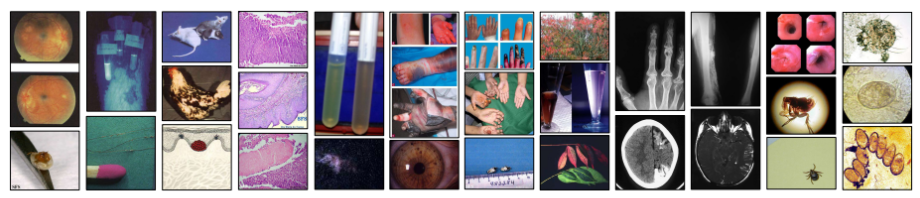
\includegraphics[width=1\textwidth]{images/fitz_erroneous.png}
      \caption{Example of erroneously included non-dermatological images.}
      \label{fig:fitz_erroneous}
    \end{figure}
  \item \textbf{Non-standard partitioning and imaging conditions:} The dataset lacks a rigorously defined held-out test set and consistent imaging environments. There are significant variations in disease presentation, field of view, illumination, and the presence of artifacts such as clothing, non-uniform backgrounds, and watermarks. These inconsistencies hinder reproducibility and model generalization (see \figurename~\ref{fig:non_standard_splits}).
    \begin{figure}[h!]
      \centering
      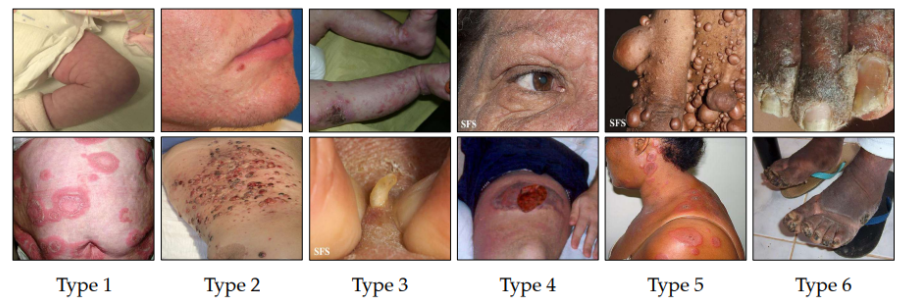
\includegraphics[width=1\textwidth]{images/fitz_partitioning.png}
      \caption{Illustration of flawed data partitioning.}
      \label{fig:non_standard_splits}
    \end{figure}
\end{itemize}

All these points, in addition to its massive size (of 16,577 images) made Fitzpatrick17k a very difficult dataset to work with.

\subsubsection{DermaMNIST}

\begin{itemize}
  \item \textbf{Data duplication:} A substantial fraction of the 10,015 images in DermaMNIST were near‐identical, originating from multiple captures of the same lesion under slightly varying orientations or magnifications \cite{pakzad}.
  \item \textbf{Mislabeled images:} Numerous instances of incorrect diagnostic labels and Fitzpatrick phototype assignments were identified, undermining the reliability of supervised learning targets \cite{abhi}.
  \item \textbf{Erroneous inclusions:} Several non‐dermatological images (e.g., artifacts, benign skin markings) were mistakenly incorporated, further introducing noise into the training distribution \cite{pakzad,abhi}.
  \item \textbf{Non‐standard partitioning:} The original release lacked a rigorously defined held‐out test set, impeding fair benchmark comparisons and inflating performance estimates \cite{abhi}.
\end{itemize}

More alarmingly, detailed lesion‐level analyses uncovered extensive data leakage across splits:

\begin{itemize}
  \item 886 images (641 unique lesions) duplicated between training and test sets,
  \item 440 images (332 lesions) between training and validation sets,
  \item 128 images (113 lesions) between validation and test sets,
  \item 51 images (40 lesions) appearing in all three partitions \cite{pakzad}.
\end{itemize}

Such leakage artificially boosts reported accuracy, masking true generalization performance and exacerbating diagnostic bias against darker phototypes (Fitzpatrick Types III–VI) prevalent in Indian cohorts.  \par

Several studies have shown that the convolutional neural networks when trained for dermatological classification perform considerably less accurately on darker Fitzpatrick phototypes (Types IV–VI) as compared to their lighter counterparts (Types I–III).~\cite{abhi} indicate that, after controlling for training set size, models trained on lighter skin images performed better than those trained on darker skin by as much as 15\% in overall diagnostic accuracy, a difference explained by two key factors: (1) higher heterogeneity of lesion morphology within darker phototypes, and (2) lower contrast between lesion and surrounding skin areas, which degrades feature extraction in conventional color‐based representations~\cite{abhi}. This shortfall is especially significant for Indian populations, in which darker skin is the prevalent skin complexion, as it can worsen delays in misdiagnosis and result in lower clinical outcomes.

\subsubsection{Dataset Corrections and New Benchmarks}
To address these biases, Abhishek et al.~\cite{abhi} introduced three rigorously curated datasets:
\begin{itemize}
    \item \textbf{DermaMNIST-C}: By grouping images by unique lesion ID and enforcing non-overlapping partitions, DermaMNIST-C eliminates the extensive train–test leakage (e.g., > 800 duplicated lesion images across splits) present in its predecessor.
    \item \textbf{DermaMNIST-E}: Extends DermaMNIST-C with additional, high-quality images drawn from the ISIC 2018 Challenge for both validation and test sets, thereby enhancing diversity in both phototype and pathology.
    \item \textbf{Fitzpatrick17k-C}: Builds on the original 17k image corpus by removing duplicated and mislabeled cases, standardizing imaging conditions, and adopting lesion-level split protocols to ensure true held-out evaluation. The authors demonstrate that models trained on these cleaned datasets exhibit a 10–12\% lift in balanced accuracy on darker skin types, narrowing—but not fully closing—the performance gap.
\end{itemize}

For our work, we plan on using \textbf{Fitzpatrick17k-C} for further development. 

\subsection{Total Body Mapping}

To ensure a comprehensive checkup of an individual, we follow the Total Body Photography (TBP) procedure proposed by Barcaui et al.~(2021)~\cite{tbp}. For patients at increased risk of melanoma, digital total-body photography captures the entire skin surface in standardized poses (front, back, both sides, arms overhead, legs apart), enabling follow-up comparisons and detection of new or evolving lesions.

\paragraph{Head \& Neck:} Face, scalp (partitioned in several strips), ears, and neck.
\paragraph{Torso:} Chest and abdomen (front); upper and lower back.
\paragraph{Upper Extremities:} Shoulders, upper arms, forearms, and hands—including palms, interdigital spaces, and nails.
\paragraph{Lower Extremities:} Thighs, lower legs, and feet—including soles, interdigital spaces, and toenails.

\subsubsection*{Standardized Dermoscopic Views}
For each suspicious lesion, the following images should be captured in order:

\begin{enumerate}
    \item \textbf{Global view:} Lesion and surrounding skin at approximately 15 - 30cm to document the site.
    \item \textbf{Regional view:} Approximately 5 - 10cm to show lesion context.
    \item \textbf{Close-up dermoscopic image:} $\leq$2 cm field of view using both polarized and non-polarized light to reveal subsurface structures.
\end{enumerate}


\section{Pharyngoscopy}

Pharyngoscopy is a medical examination technique used to visualize the pharynx (throat) and adjacent structures. Clinically, this is most commonly performed by a physician shining a bright light into the patient`s mouth, sometimes using a small mirror or a fiberoptic scope to inspect the throat.~\cite{onto} This procedure is non-invasive and typically performed in an outpatient setting. \par

The viability of telemedicine for laryngological diagnosis was proven in a seminal study that evaluated concordance rates between pre-laryngoscopy telemedicine encounters and follow-up in-person assessments with laryngoscopy.~\cite{choi} Research has shown high reliability and accuracy in diagnosing various otolaryngological conditions, including otologic conditions, rhinosinusitis, peritonsillar abscess, and nasal fractures through telemedicine platforms. While direct laryngoscopy remains the gold standard for definitive diagnosis, telemedicine consultations have proven effective for initial assessment and empiric management until in-person laryngoscopy can be performed. \par

The structure and dimensions of the pharynx are not uniform across all individuals, and emerging evidence indicates that these anatomical characteristics can indeed vary based on race and ethnicity. A significant study by Kollara et al. (2014) investigated the craniometric and velopharyngeal anatomy of young children aged 4 to 8 years from Black and White racial groups.~\cite{kollara} However, the difference is not as stark as it was in dermatoscopic scans, which is why we have left racial agnostism for furture scope in this solution.

\subsection{Dataset}

The Pharyngitis Dataset (v4) on Roboflow Universe comprises 559 annotated images evenly distributed across two classes: \emph{phar} and \emph{nophar}~\cite{robo}.

All images are auto-oriented and statically cropped to the central 25–75\% region, focusing on pharyngeal anatomy; they are then resized to 640 x 640 pixels for input consistency. Data augmentation via horizontal and vertical flips, 90° rotations, and random crops (0–20\% zoom) doubles the training set, reflecting common strategies in medical imaging to improve generalization. \par

The dataset adopts an 82\%–12\%–\% split (460/66/33 images) for training, validation, and testing, respectively \cite{robo}. While the validation proportion aligns with best practices for medium-sized datasets \cite{encord2024}, the small test set (N = 33) may reduce statistical power and inflate variance in final metrics \cite{wilb}. Although stratified sampling is generally recommended to preserve class balance \cite{encord2024}, explicit mention of its implementation here is absent.

Targeted cropping minimizes background noise and isolates relevant anatomical features \cite{encord2024}. Augmentation strategies simulate clinical variability in imaging angles and scales, critical for robust performance across heterogeneous real-world settings \cite{wilb}. The binary class balance facilitates initial model convergence without severe imbalance, a common practice in early-stage classification benchmarks \cite{radimagenet2021}.

\begin{figure}
    \centering
    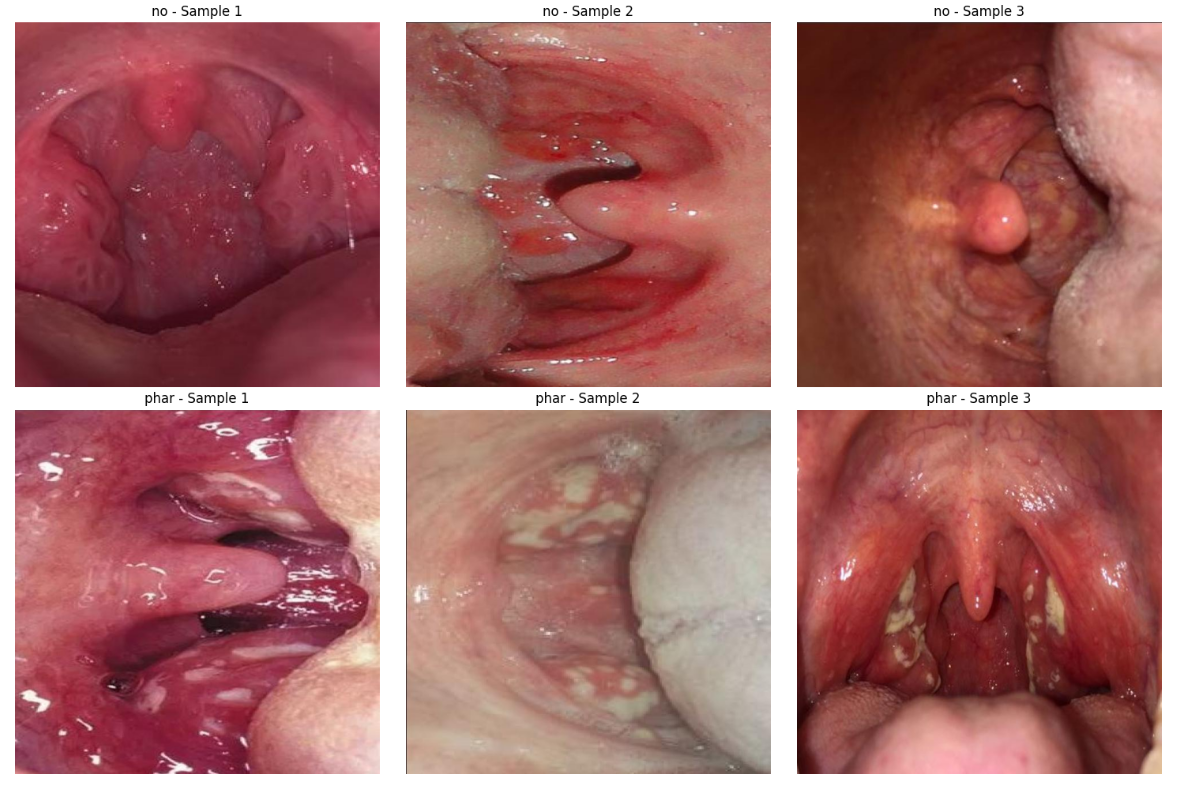
\includegraphics[width=1\textwidth]{images/roboflow_samples.png}
    \caption{Sample of a few images from the Roboflow Pharyngitis Dataset (v4).}
    \label{fig:roboflow_samples}
\end{figure}

Absence of metadata regarding acquisition modalities (e.g., endoscopic vs. smartphone imaging) hinders assessment of domain shift and generalization \cite{wilb}. Labeling protocols—including inter-rater reliability measures—are unspecified, raising concerns about annotation consistency \cite{encord2024}. Finally, the overall sample size (N = 559) remains modest compared to large-scale medical imaging collections, emphasizing the need for expanded, multi-center datasets \cite{robo}.

\subsection{Existing Solutions}

A significant technical advancement in pharyngoscopy was seen in Nakojo et. al. (2023). It involves AI-based anatomical classification of endoscopic images. Researchers developed a neural network trained on 5,382 endoscopic images to classify pharyngeal and laryngeal regions into 15 distinct anatomical locations. This system achieved 93.3\% overall accuracy with weighted averages of 0.934 for precision, 0.933 for recall, and 0.933 for F1-score when evaluated on an independent dataset of 1,110 images. The technical implementation employed gradient-weighted class activation mapping (Grad-CAM) \cite{selva} and Guided Grad-CAM, both by Selvaraju et. al., to visualize the specific image regions informing the algorithm's classifications. This approach provides transparency into the AI's decision-making process and helps identify potential blind spots during examinations, thereby improving diagnostic thoroughness~\cite{nakajo} \par

In our work, we explore the possibility of ViTs (Vision Transformers) in this line of disease detection as a novel approach to pharyngitis detection.

\section{Otoscopy}

A meta-analysis and systematic review of AI models for otoscopic image classification showed considerable diagnostic performance across different algorithmic strategies. Technical methods compared were convolutional neural networks (CNNs), artificial neural networks, support vector machines, decision trees, and k-nearest neighbors algorithms. The models were trained to differentiate among several diagnostic classes, namely normal tympanic membrane, acute otitis media, otitis media with effusion, chronic otitis media with/without perforation, cholesteatoma, and ear canal obstruction.

Performance analysis demonstrated that AI algorithms achieved 90.7\% (95\% CI: 90.1-91.3\%) accuracy in binary classification (normal vs. abnormal) across 14 studies. More sophisticated multiclass algorithms achieved 97.6\% (95\% CI: 97.3-97.9\%) accuracy in differentiating between normal, acute otitis media, and otitis media with effusion. Notably, when directly compared with human diagnosticians, AI systems demonstrated superior performance, achieving 93.4\% (95\% CI: 90.5-96.4\%) accuracy versus 73.2\% (95\% CI: 67.9-78.5\%) for human assessors. Among the various technical approaches, CNNs consistently achieved the highest diagnostic accuracy. 